\section {Grundlagen}
\subsection{ROS2}
\ac{ROS2} ist eine Sammlung von Bibliotheken und Werkzeugen für Robotik-Applikationen welche alle OpenSource sind.
Die erste \ac{ROS2} Release-Version erschien im Dezember 2017 unter dem Namen Ardent Apalon \citet{ros2docs}.\\
Es werden  mehrere \acp{RCL}  zur Verfügung gestellt, welche den Zugriff auf die \ac{ROS2}-API ermöglichen.
Die \acp{RCL} für die Sprachen C++ und Python (rclcpp und rclpy) werden dabei direkt vom \ac{ROS2}-Team verwaltet.
Von der Community wurden weitere \acp{RCL}, unter anderem für die Sprachen C\#, Swift und Rust, entwickelt.\\
Um die Entwicklung der \acp{RCL} zu vereinfachen und die Logik sprachen unabhängig zu machen werden Funktionalitäten als C Interfaces zugänglich gemacht, für welche in den \acp{RCL} Wrapper geschrieben werden.
\subsubsection{Node}
Nodes sind die grundlegenden Komponenten, aus welchen eine \ac{ROS2} Anwendung besteht.
Typischerweise besteht eine Anwendung aus mehreren Nodes.
Entsprechend dem Prinzip Separation of Concerns (Trennung der Zuständigkeiten) sollen Nodes so implementiert werden, dass sie jeweils nur eine spezifische Aufgabe haben.
\subsection{ROS2 Interfaces}
In diesem Abschnitt werden die verschiedenen Arten von Interfaces beschrieben, welche für die im folgenden Abschnitt~\ref{rosnodecomm} erklärten Methoden zur Kommunikation zwischen mehreren Nodes genutzt werden.\\
\ac{ROS2} Interfaces sind Definitionen, welche Daten mit welchen Typen gesendet werden.
Sie werden in der \ac{IDL} geschrieben, welche es ermöglicht automatisch Source Code in verschiedenen Sprachen für diese zu generieren.\\
- Erklären was für den build nötig ist?
\subsubsection{Message}
Eine Message ist der einfachste Typ der \ac{ROS2} Interfaces, welcher gleichzeitig auch ein Baustein für die folgenden Interfaces sein wird.\\
Message Definitionen haben die Dateiendung \verb|.msg| und werden per Konvention in einem Ordner \verb|msg/| gespeichert.
Jede \verb|.msg| Datei besteht aus den folgenden Teilen:
\begin{itemize}
\item Felder
\item Konstanten
\end{itemize}
Jedes Feld besteht aus einem Typ und einem durch ein Leerzeichen getrennten Namen: \verb|typ name|, z.B. \verb|bool isDone|.
Als Typ können dabei die integrierten Typen (s. Tabelle~\ref{tab:builtintypes}) oder der Name anderer Messages genutzt werden.
Zusätzlich kann jeder integrierte Typ als Array definiert werden (s. Tabelle~\ref{tab:arraytypes}).\\
Feldnamen müssen kleingeschrieben sein.
Es können alphanumerische Zeichen sowie der Unterstrich zur Trennung von Wörtern genutzt werden.
Das erste Zeichen muss ein Buchstabe sein und der Name darf nicht mit einem Unterstrich enden.
Zusätzlich darf es keine aufeinander folgenden Unterstriche geben.\\
Konstanten behalten das Format der Felder bei.
Der Name der Konstante wird komplett in Großbuchstaben geschrieben.
Zusätzlich bekommen Konstanten einen Wert zugewiesen, welcher nicht innerhalb des Programms geändert werden kann.
Die Zuweisung des Wertes erfolgt mit dem \verb|=| Zeichen: \verb|string EXAMPLE="test"|.
\begin{table}[ht]
    \centering
    \caption{Integrierte Datentypen für Interfaces und deren C++ Equivalent}
\begin{tabular}{|l|l|}
\hline
\textbf{Typ} & \textbf{C++}   \\ \hline
bool         & bool           \\ \hline
byte         & uint8\_t       \\ \hline
char         & char           \\ \hline
float32      & float          \\ \hline
float64      & double         \\ \hline
int8         & int8\_t        \\ \hline
uint8        & uint8\_t       \\ \hline
int16        & int16\_t       \\ \hline
uint16       & uint16\_t      \\ \hline
int32        & int32\_t       \\ \hline
uint32       & uint32\_t      \\ \hline
int64        & int64\_t       \\ \hline
uint64       & uint64\_t      \\ \hline
string       & std::string    \\ \hline
wstring      & std::u16string \\ \hline
\end{tabular}
    \label{tab:builtintypes}
\end{table}
\begin{table}[ht]
    \centering
    \caption{Array Typen und deren C++ Equivalent}
\begin{tabular}{|l|l|}
\hline
\textbf{Typ} & \textbf{C++}   \\ \hline
static array               & std::array<T, N>   \\ \hline
unbounded dynamic array    & std::vector        \\ \hline
bounded dynamic array      & custom\_class<T, N> \\ \hline
bounded string             & std::string        \\ \hline
\end{tabular}
    \label{tab:arraytypes}
\end{table}
\subsubsection{Service}
Service Definitionen beschreiben eine Anfrage und eine Antwort.
Die Definition hat die Dateiendung \verb|.srv| und wird im Ordner \verb|srv/| gespeichert.
Anfrage und Antwort werden innerhalb der Datei durch \verb|-| getrennt.
Für beide Teile gilt, dass sie gültig sind, wenn sie einer gültigen Message Definition entsprechen.
Ein Beispiel einer einfachen Servicedefinition ist in Listing~\ref{lst:serviceexample} zu sehen.\\
\begin{minipage}{\linewidth}%minipage to prevent page break
\begin{lstlisting}[caption={Beispiel einer Service Definition}, label={lst:serviceexample}]
int32 request_int
string request_string
---
float32 response_float
\end{lstlisting}
\end{minipage}
\subsubsection{Action}
Action Definitionen bestehen aus den 3 Teilen Anfrage, Ergebnis und Feedback, in dieser Reihenfolge.
Wie auch für Service Definitionen gilt, das die Teile durch \verb|-| getrennt sind und jeder einzelne Teil gültig ist, wenn er einer gültigen Message Definition entspricht.
\subsection{ROS2 Node Kommunikation}{\label{rosnodecomm}}
Damit verschiedene Nodes untereinander kommunizieren können, gibt es verschieden Mechanismen, welche sich primär darin unterscheiden, in welche Richtungen Nachrichten gesendet werden und ob es eine direkte Reaktion gibt.
Für alle Mechanismen gilt, das sie von einer Node unter einem bestimmten Namen sowie einem Typ zur Verfügung gestellt werden und von anderen Nodes durch eben diese genutzt werden können.
\subsubsection{Topic}
Topics entsprechen in etwa einem Newsletter System: eine Node veröffentlicht Daten, welche von allen anderen Nodes empfangen wird, die sich für diese registriert haben.
Das Format der Daten entspricht einer gewählten Message Definition.
\subsubsection{Service und Client}
Services werden für Prozesse genutzt, in denen eine Anfrage gesendet und eine Antwort erwartet wird.
Als Typ wird eine Servicedefinition genutzt.
\subsubsection{Action Server und Client}
Actions sind für länger andauernde Prozesse gedacht.
Eine Node erstellt einen Action Server über welchen eine Action zur Verfügung gestellt wird.
Andere Nodes können über einen Action Client eine Anfrage senden.
Der Server bearbeitet die Anfrage und sendet bei Beendigung eine Antwort mit einem Ergebnis an den Client.
Während der Dauer der Action kann der Server den Client optional mit Feedback Nachrichten über den aktuellen Status informieren.\\
Als Typ wird eine Action Definition genutzt. 
\subsection{OpenMANIPULATOR-X}
Der OpenMANIPULATOR-X ist ein von der Firma ROBOTIS{\footnote{http://en.robotis.com}} nach den Prinzipien ``OpenSoftware`` und ``OpenHardware`` hergestellter Greifarm.
OpenSoftware steht hierbei dafür, dass es ein OpenSource Projekt ist und auf dem OpenSource Projekt \ac{ROS2} basiert.
OpenHardware steht dafür, dass die meisten Komponenten als STL-Dateien zur Verfügung stehen und als Ersatzteile oder zum Anpassen des Greifarms mittels eines 3D-Druckers selbst hergestellt werden können.\\
Der OMX(Greifarm?,Abk?) ist eine 5DOF (5 Degrees of Freedom) Plattform, welche mittels 5 Servomotoren{\footnote{DYNAMIXEL XM430-W350-T}} gesteuert wird.
Dies ist aufgeteilt in 4DOF für den Arm sowie 1DOF für den Greifer.
Es kann eine Last bis 500g getragen werden
\subsection {Planung}
Planung (auch Handlungsplanung) ist ein Bereich der Künstlichen Intelligenz, welcher sich mit der Lösung von Planungs- und Schedulingproblem befasst~\cite{aiplanning}.
\subsubsection{Stanford Research Institute Problem Solver}
Der \ac{STRIPS} ist ein automatischer Planer, welcher von Richard Fikes und Nils Nilsson 1971 entwickelt wurde~\cite{FIKES1971189}.
Mit dem gleichen Namen wird auch die Sprache bezeichnet, welche als Eingabe für diesen Planer genutzt wird.
In diesem Abschnitt wird nur auf die Sprache eingegangen, welche die Grundlage vieler weiterer Sprachen zur Darstellung von Planungsdomänen und -problemen ist.\\
Ein \ac{STRIPS}-Modell besteht aus 3 Teilen:
\begin{itemize}
    \item Startzustand
    \item Zielzustand
    \item Aktionen
\end{itemize}
Aktionen bestehen wiederum aus:
\begin{itemize}
    \item Vorbedingungen
    \item Effekten
\end{itemize}
Ein \ac{STRIPS}-Modell kann außerdem mathematisch als 4-Tupel \((P,I,O,G)\) beschrieben werden:
\begin{enumerate}
    \item \(P\): eine Menge von Bedingungen
    \item \(I\):
    \item \(O\): der Startzustand, eine Menge von Bedingungen, die wahr sind
    \item \(G\): der Zielzustand, ein Paar \((N,M)\)
\end{enumerate}
Es gilt die \emph{Closed World Assumption (CWA)}: alles was nicht explizit als wahr beschrieben ist, gilt als falsch.

%Bedingungen werden als Prädikate dargestellt: \verb|Geöffnet(Baumarkt)| beschreibt die Bedingung, dass ein Subjekt \emph{Baumarkt} die Eigenschaft \emph{Geöffnet} hat.
Ein Plan besteht aus mehreren Aktionen, welche, in der gegebenen Reihenfolge ausgeführt, vom Startzustand zu einem Zustand führen, von dem der Zielzustand eine Teilmenge ist.\\
Aktionen sind 4-Tupel, bei dem jedes Element eine Menge von Bedingungen sind.
Die ersten zwei Mengen beschreiben die Vorbedingungen: Bedingungen die wahr sein müssen sowie Bedingungen, die falsch sein müssen.
Die letzten beiden Mengen beschreiben den Effekt, den die Aktion nach ihrer Ausführung auf einen Zustand hat: Bedingungen die wahr werden und Bedingungen die falsch werden.
\subsubsection{Planning Domain Definition Language}
Die \ac{PDDL} ist eine Sprache zur Modellierung von Planungs...
\subsubsection{PDDL-Plugin für VS Code}
- nach Implementierung verschieben?\\
- Installation\\
- Nutzung / Ausführung\\
- Pfad zur popf executable im foxy ordner\\
- Screenshot mit Bsp. für Planausgabe und Visualisierung\\
Im Marketplace von Visual Studio Code ist ein PDDL-Plugin von Jan Dolejsi verfügbar.
Dieses vereinfacht die Entwicklung und das Testen von Domänen und Problemen im PDDL Format.
Es beinhaltet Syntax-Highlighting und Snippets, sowie die Möglichkeit direkt Pläne zu suchen und zu visualisieren.
Um Pläne mit \ac{POPF} zu suchen, muss der Planer in der Overview-Page des Plugins hinzugefügt werden.
Der Pfad zum \ac{POPF}-Planer ist: \emph{/opt/ros/foxy/lib/popf/popf}.\\
Über das Kontext-Menü einer Domänen- oder Problemdatei lässt sich der Planer starten und es erfolgt eine Ausgabe in der Konsole (s. Abbildung~\ref{fig:pluginplan}) sowie eine Visualisierung wenn ein Plan gefunden wurde (s. Abbildung~\ref{fig:pluginvis}).
Die Visualisierung erfolgt dabei zeitlich von links nach rechts.
Alle Aktionen werden farblich markiert, wobei eine Aktion auch bei mehrfacher Ausführung die gleiche Farbe hat.
Im oberen Abschnitt gibt es eine einfache Übersicht des Plans: welche Aktionen wurden wann ausgeführt und mit welchen Parametern.
Im unteren Abschnitt wird dargestellt, welche Instanzen, zu welchem Zeitpunkt, als Teil welcher Aktion genutzt wurden.
\begin{figure}[ht!]
    \centering
    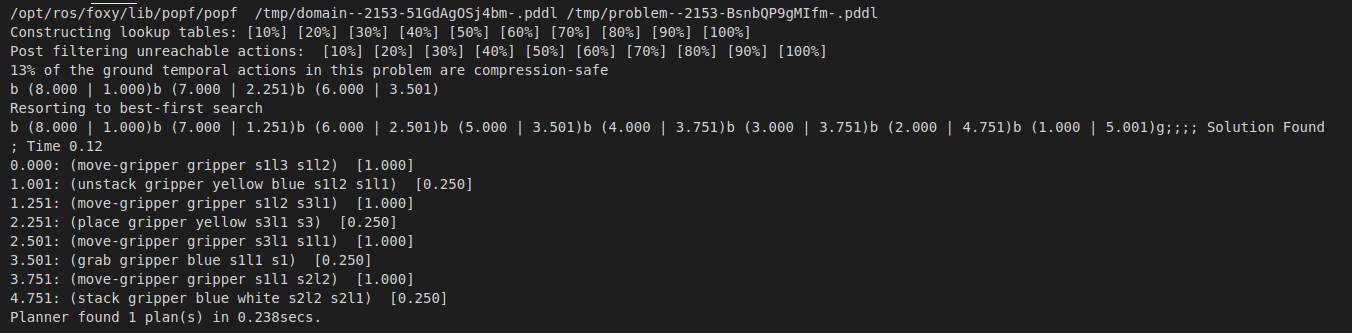
\includegraphics[width=\textwidth]{plugin_plan}
    \caption{Konsolenausgabe nach Ausführung des Planers über das PDDL-Plugin}
    \label{fig:pluginplan}
\end{figure}

\begin{figure}[ht!]
    \centering
    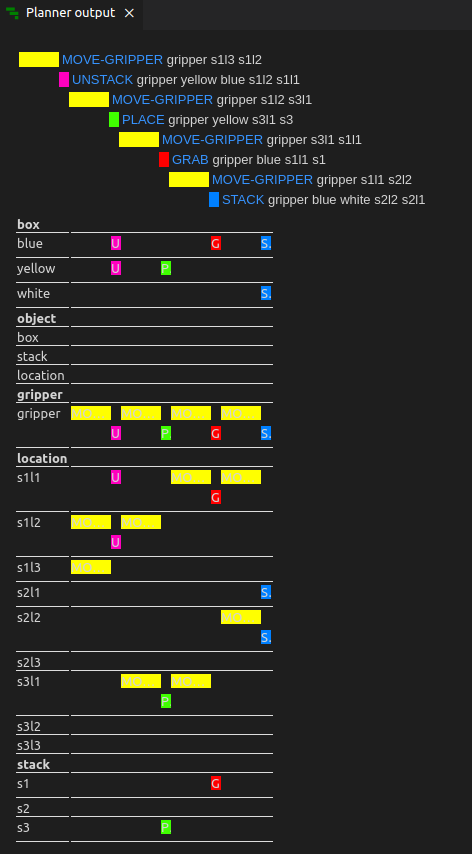
\includegraphics[width=\textwidth]{plugin_vis}
    \caption{Visualisierung eines Plans mit dem PDDL-Plugin}
    \label{fig:pluginvis}
\end{figure}
\subsubsection{Partial Order Planning}
\subsubsection{Forward Chaining Partial Order Planning}
\subsubsection{Partial Order Planning Forward}
~\citep{popf}
\subsubsection{Behavior Tree}